
\section{Test und Messung}

Am Ende der Inbetriebnahme haben wir verschieden Tests und Messungen gemacht. 
Unter anderem wurden die Ansteuersignale zweier Schalter aufgezeichnet. Man sieht gut, dass sich der Duty Cycle sinuidal verändert und es lange Aus-Zeiten gibt(ein hoher Pegel öffnet den Schalter). Die Phasenverschiebung der beiden Sinui beträgt 120 Grad, was sich aus dem Bild näherungsweise ermitteln lässt.
\begin{figure}[H]
		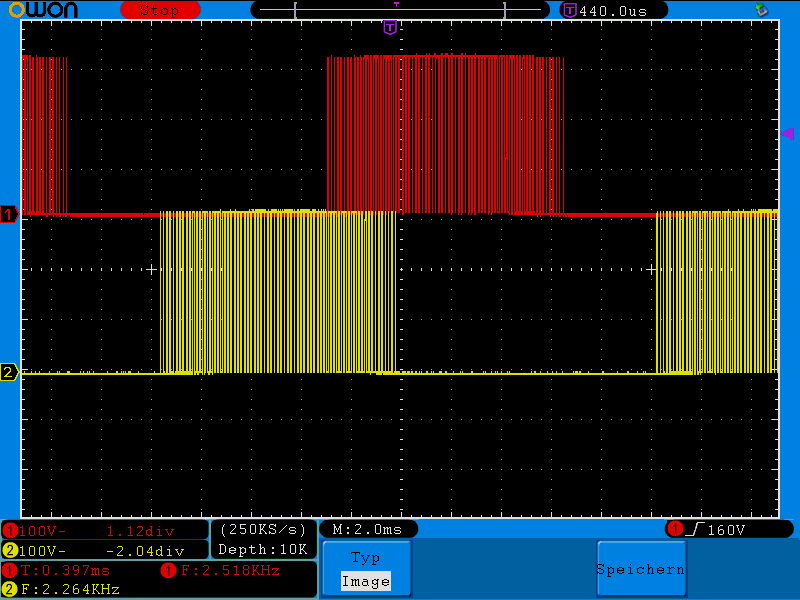
\includegraphics[width=0.5\textwidth]{uwgeregelt.png}
		\caption{Schaltmomente)}
		\label{fig:rreibChart}
	\end{figure}
	Des Weiteren wurde der Strom durch eine Phase im Leerlauf mit einer Stromzange ermittelt. Leerlauf heißt, dass die Terminals des Generators offen waren. Hierbei gilt, dass 100mV einem A entsprechen. Zu sehen sind neben mehren Messfehlern vor Allem die Sinuskurvenförmigkeit des Stroms. Messaufbaubedingt war es leider nicht möglich Spannung und Strom zum selben Zeitpunkt zu messen, wir würden dabei eine Phasenverschiebung auf Grund der Induktivität der Motorinduktivität erwarten.  
	\begin{figure}[H]
		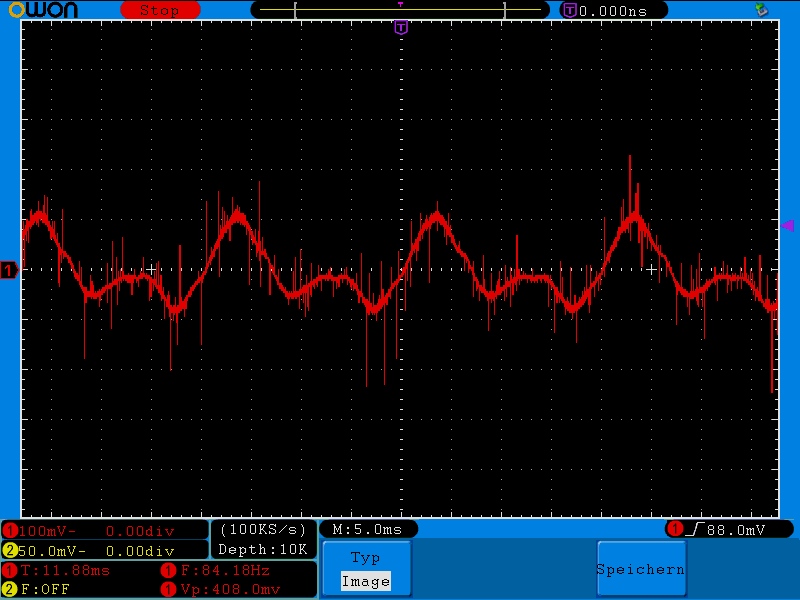
\includegraphics[width=0.5\textwidth]{strom1Phase.png}
		\caption{Zeitlicher Verlauf der Drehzahl im Vergleich zur Nenndrehzahl(hier Solldrehzahl)}
		\label{fig:rreibChart}
	\end{figure}